\chapter{绪论}

\section{课题来源}
红外目标检测指的是利用红外探测器感知目标和背景之间的红外辐射差异成像后进行目标检测的过程。可见光图像虽然具有成像分辨率高、目标细节信息丰富等特点,但其相比于红外图像很容易受到光照变化的影响,这在很大程度上增加了目标识别的难度。尤其是在一些特殊天气,例如雨天、雾天、夜间和可见光光源缺少的情况下,可视距离和能见度很差,拍摄的图片根本无法正常使用。而红外成像技术具有工作距离远、抗干扰能力强、测量精度高、受天气影响较小、能昼夜工作及穿透烟雾能力强等特点,因此红外成像技术一经提出来便得到科研领域和民用领域的广泛关注,市场对红外目标检测的需求也随之增加。红外目标检测不仅应用于军事领域,在工业、安防、交通等民用领域也有着广泛的应用。例如红外技术可以应用于无人驾驶车上进行全天候的目标检测;在工业方面,红外技术能够检测出器件是否出现接触不良或损坏;尤其在今年疫情期间,红外技术广泛应用在火车站机场等人流密集的场所,能够实时的检测体温,避免了人工检测体温造成的拥堵。

本课题主要研究红外图像中的无人机检测算法。本课题来源于哈尔滨海邻科信息技术有限公司“警用人工智能技术合作”。当前,无人机市场呈现井喷式发展,给社会带来极大便利的同时,无人机的“肇事”事件也呈逐年上升趋势。国外机场无人机扰航事件频发,国内各地无人机“黑飞”也引起军内外广泛关注,给机场安全维护、反恐维稳和国家边境防护等工作带来很大压力,迫切需要通过对无人机的探测来对无人机施行监控和预警。在无人机探测中,基于声、无线电和雷达探测的技术较为常见,但这些技术往往需要昂贵的设备和严格的配置。基于机器视觉的方法具有成本低、配置简单等优点,随着深度学习技术的发展,已逐步应用于各类目标的识别和检测。然而无人机通常低空飞行,又有光照、遮挡物等的影响,检测场景十分复杂,且体积小、速度快,一直是目标检测领域的难题。相关的监管部门需要部署相应的探测网络,用以及时发现监管区域内的非法无人机,以保证群众的人身安全和财产安全。因此本课题的目标就是研究设计一种快速有效的红外图像无人机检测算法。

\section{研究背景与意义}
计算机视觉技术是一种让计算机从给定的图像或视频中获取相关信息并进行“感知”的技术,是人类视觉感知的扩展。半导体行业促进了硬件水平的提高,也带动了机器视觉的发展,使其在人工智能领域得到广泛应用。

在计算机视觉领域中,基于红外探测系统的红外弱小目标检测一直都是一个重要的课题和研究热点。当前主流的探测系统可分为3类:可见光探测、红外成像探测和雷达探测系统。红外探测系统只对目标的温度与本身的材料特性敏感,而与环境等因素无关,使得其在3类探测系统中脱颖而出,具有一系列优势:
(1)不受光照的影响,可以全天时工作;
(2)由于其不发射电磁波,因此是非自动的探测方法;
(3)穿透能力强,可以避免灰尘、云层和烟雾等的遮挡,可以更好地识别虚假的伪装目标。以上优势也使其成为传统可见光探测系统与雷达探测系统的有效补充或替代。

随着红外探测系统性能的不断提高,红外探测技术已经广泛应用于红外预警、搜索潜艇和红外制导等军事领域以及医学病变细胞诊断和工业探伤等民用领域,并取得了显著成就。在军事和医疗等民用领域中,高检测率、低虚警率的实时红外小目标检测是实际应用的必然需求。然而,在大多数实际应用的红外成像系统中,待检测目标与探测器之间的距离较远,使得红外目标占整幅红外图像的面积非常小,一般少于100个像素,加上背景复杂多变的特点,为检测带来困难。具体表现为以下几点:
(1)红外目标的特点:红外弱小目标本身缺乏颜色和纹理等特征,尺寸小(一般小于9×9个像素),大多数方法只能利用其灰度分布特征、运动特征以及运动方向等特征。此外,红外小目标的信噪比低,容易被复杂多变的背景以及云层海波中的噪声所淹没。
(2)红外背景的特点:背景相似,分布连续;目标经常存在于云层、海浪中,场景复杂多变;复杂的红外图像背景特征表现较为不均匀,相对于目标区域的灰度较暗。
(3)红外目标检测的难点:1)目标可用特征少。由于目标尺寸小,总辐射能量小于背景的辐射能量,在图像中灰度分布多变,难以采用统一的数学模型进行描述;且不存在精细的纹理、形状等结构信息,使得传统可见光图像的目标检测方法无法直接用于红外弱小目标检测中。2)图像的信噪比低。由于成像距离远,使得小目标与云层、海浪等的杂波和噪声有相似的特点,进而易被淹没和干扰,从而导致小目标的强度小,图像的信噪比低,目标信号几乎淹没在难以预测的背景中,更加难以检测。3)检测准确率不高。在实际情况和应用中,目标的运动方向和速度具有高机动性,这也使得提高机动目标的检测准确率成为学者们致力解决的问题。4)成像环境复杂。在红外精确制导和预警方面,成像过程中往往伴随着烟雾和海波等,这对不同检测算法的鲁棒性提出了更高的要求。5)实时性差。检测效果通常与计算量近似反比,检测效果好的算法往往计算量大,因为建模量大、计算硬件条件跟不上,导致实时性差。6)公开的数据集少。红外小目标检测大多用于军事领域,存在一定的保密性,供研究者公开使用的红外数据库很少,这也在一定程度上制约了小目标检测算法的发展。本课题要进行检测的目标图像如图\ref{uav}所示。

\begin{figure}[htbp]
    \centering
    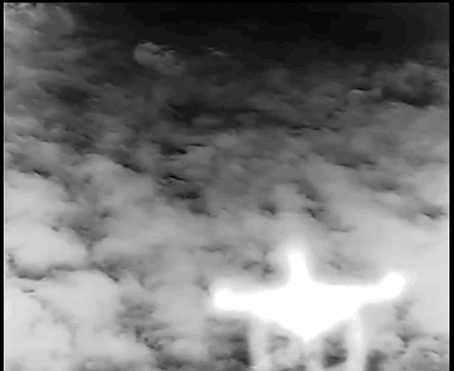
\includegraphics[width = 0.8\textwidth]{无人机目标示例.png}
    \caption{无人机目标示意图}
    \label{uav}
\end{figure}

综上所述,红外图像的目标检测应用广泛,具有很大的研究价值。本文基于深度学习算法,针对红外无人机目标进行研究,针对红外图像无人机目标检测的特点,从数据增强、网络结构改进、网络轻量化、嵌入式实现这四个方面展开研究。

\section{国内外研究发展现状}
目标检测包括目标分类和目标定位两个子任务,用于检测视频中特定类别的语义对象实例。本文从传统的目标检测、基于深度学习的two-stage目标检测算法、基于深度学习的one-stage目标检测算法三个阶段介绍目标检测算法的发展过程\cite{尹宏鹏2016基于视觉的目标检测与跟踪综述}。

\subsection{传统的目标检测算法}
如图\ref{ct}所示,传统的目标检测算法流程是先选定目标区域,经过特征提取之后通过分类器分类得到检测结果。

\begin{figure}[htbp]
    \centering
    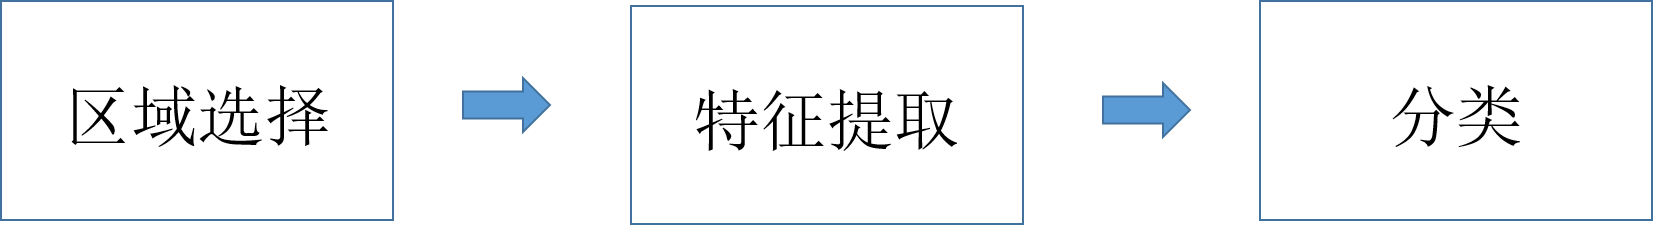
\includegraphics[width = 0.9\textwidth]{传统目标检测.png}
    \caption{传统目标检测流程}
    \label{ct}
\end{figure}

在传统的目标检测算法中,最初区域选择采用不同尺度长宽比的滑动窗口遍历整幅图像,框出候选区域即可能包含目标的区域\cite{胡伏原2020基于卷积神经网络的目标检测算法综述,kira1992feature}。这种穷举的方法时间复杂度高,会产生大量冗余窗口,会影响之后的特征提取及分类的速度和精度。后来发展出更加高效的区域选择算法,如Selective Search\cite{uijlings2013selective},  Edge Boxes\cite{zitnick2014edge}等。Selective Search将图片划分成很多的小区域,然后根据计算得到的两两区域之间的相似度及区域的大小不断地聚合相邻的小区域,重复上述过程直到整张图片组合成一个大的区域。Edge Boxes利用edge group之间的相似性,根据权值判断box中包含的轮廓数或与box边界重叠的轮廓数,基于以上信息对box进行打分,然后根据box得分的高低顺序确定候选区域的信息。第二步从候选区域提取固定长度的特征向量,来获取此区域的判别语义信息。传统的机器学习采用手工特征作为机器学习模型的输入,目标检测领域也是如此。但是由于目标的形态多种多样,光照变化及背景的多样性等因素使得设计一种鲁棒的特征不是很容易,并且提取到的特征好坏直接影响到之后分类的准确性。在这一阶段,常用的图像特征有HOG特征和SIFT特征等。HOG将图像分割成一个个小的连通区域(细胞单元),在每个单元内部采集每个像素点的梯度或边缘的梯度直方图,得到的直方图就是这个单元的特征。SIFT特征提取算法首先对输入的图像在DoG尺度空间上提取极值点,然后对尺度空间DoG函数进行拟合,进行关键点的精确定位,去除不稳定的关键点。然后计算剩余的关键点的主方向,构造SIFT描述子。SIFT特征由于其具有尺度、旋转不变性,并且能够适应复杂的光照变化,因此常用于传统的目标检测领域。第三步提取特征之后,用分类器进行分类,分类算法有Adaboost算法和SVM分类器。传统的目标检测算法主要存在以下两个问题:一是计算的复杂度高,区域选择策略没有针对性,具有窗口冗余,会导致后续分类过程出现错检的现象;二是手工设计的特征对于环境多样性没有很好的鲁棒性,对于复杂环境情况下手工设计的特征没有办法获取准确的语义信息,检测的精度不高。相对于传统的目标检测算法,深度卷积神经网络能够从训练数据的过程中自动的获取图像中的层次特征表示,如低层次的卷积获取位置信息,高层次的卷积获取目标语义信息。同时如果使用的数据集越大学习到的信息更多,表示能力越强。因此在卷积神经网络提出后,基于卷积神经网络的目标检测算法快速发展,相比于传统算法表现出很多优势。
\section{本文主要研究内容}

\section{本文组织结构}